
% !TEX TS-program = pdflatex
% !TEX encoding = UTF-8 Unicode

% This is a simple template for a LaTeX document using the "article" class.
% See "book", "report", "letter" for other types of document.

\documentclass[11pt]{article} % use larger type; default would be 10pt

\usepackage[utf8]{inputenc} % set input encoding (not needed with XeLaTeX)

%%% Examples of Article customizations
% These packages are optional, depending whether you want the features they provide.
% See the LaTeX Companion or other references for full information.

%%% PAGE DIMENSIONS
\usepackage{geometry} % to change the page dimensions
\geometry{a4paper} % or letterpaper (US) or a5paper or....
% \geometry{margin=2in} % for example, change the margins to 2 inches all round
% \geometry{landscape} % set up the page for landscape
%   read geometry.pdf for detailed page layout information

\usepackage{graphicx} % support the \includegraphics command and options

% \usepackage[parfill]{parskip} % Activate to begin paragraphs with an empty line rather than an indent

%%% PACKAGES
\usepackage{booktabs} % for much better looking tables
\usepackage{array} % for better arrays (eg matrices) in maths
\usepackage{paralist} % very flexible & customisable lists (eg. enumerate/itemize, etc.)
\usepackage{verbatim} % adds environment for commenting out blocks of text & for better verbatim
\usepackage{subfig} % make it possible to include more than one captioned figure/table in a single float
% These packages are all incorporated in the memoir class to one degree or another...

%%% HEADERS & FOOTERS
\usepackage{fancyhdr} % This should be set AFTER setting up the page geometry
\pagestyle{fancy} % options: empty , plain , fancy
\renewcommand{\headrulewidth}{0pt} % customise the layout...
\lhead{}\chead{}\rhead{}
\lfoot{}\cfoot{\thepage}\rfoot{}

%%% SECTION TITLE APPEARANCE
\usepackage{sectsty}
\allsectionsfont{\sffamily\mdseries\upshape} % (See the fntguide.pdf for font help)
% (This matches ConTeXt defaults)

%%% ToC (table of contents) APPEARANCE
\usepackage[nottoc,notlof,notlot]{tocbibind} % Put the bibliography in the ToC
\usepackage[titles,subfigure]{tocloft} % Alter the style of the Table of Contents
\renewcommand{\cftsecfont}{\rmfamily\mdseries\upshape}
\renewcommand{\cftsecpagefont}{\rmfamily\mdseries\upshape} % No bold!

\makeatletter
   \newcommand\figcaption{\def\@captype{figure}\caption}
   \newcommand\tabcaption{\def\@captype{table}\caption}
\makeatother
%%% END Article customizations

%%% The "real" document content comes below...

\title{CSE 509 Lecture 5}

\author{Prof. Rob Johnson, Scribe:Arun Rathakrishnan}
%\date{} % Activate to display a given date or no date (if empty),
         % otherwise the current date is printed 

\begin{document}
\maketitle

\section{Review - Buffer Overflow}
\subsection{Code Injection Attack}
Causing a program to violate trust, by providing input which causes a buffer to
overflow, thereby forcing the machine to execute untrusted code.

\subsection{Set up}
\begin {itemize} \itemsep -2pt
\item Consider a machine in which the activation records (arguments local
variables and return address for a function which is being called) are stored on
a stack. The machine executes code in a page which contains the address pointed
to by the Instruction Pointer ($IP$). $IP$ can also point to a byte in stack segment.
\item A local variable allocated in stack, can point to a buffer allocated in stack.
When the user input is used to fill up contents of the buffer, the input can overwrite
parts of stack that contain the return address and arguments from the caller and beyond.
\item By providing a malicious input overwriting the return address
of the current function to the beginning of the malicious program on the stack,
an attacker can force the machine to jump after the execution of the vulnerable 
function, to the beginning of a malicious program in stack and start executing it.
\end {itemize}

\subsection{How to prevent?}
Use NX (Non-executable) bit to mark pages that are not executable. Only pages
in the text section of a process are executable. Stack section has NX bit set.
So even if control is transferred to the stack by changing the IP, the system
will be forced to page fault and terminate the process.

\subsection{VM Layout}
\begin{center}
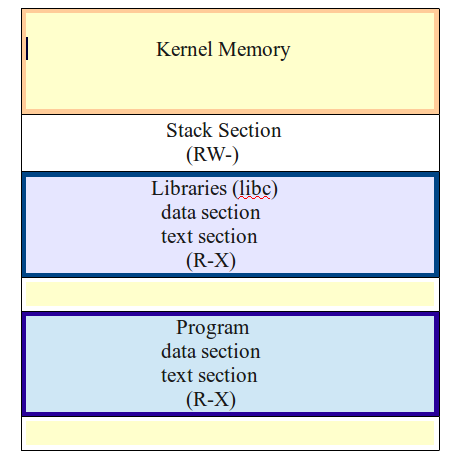
\includegraphics [width=200px,height=220px] {img/img1.png}
\end{center}

\subsection{Activation Records in Stack}
\begin{center}
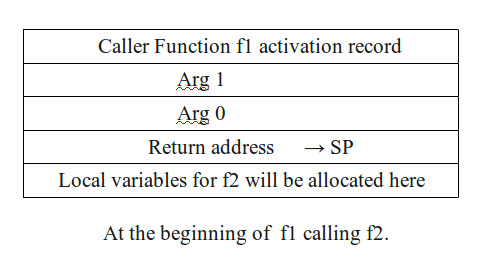
\includegraphics [width=200px,height=120px] {img/img2.png}
\end{center}
\begin{center}
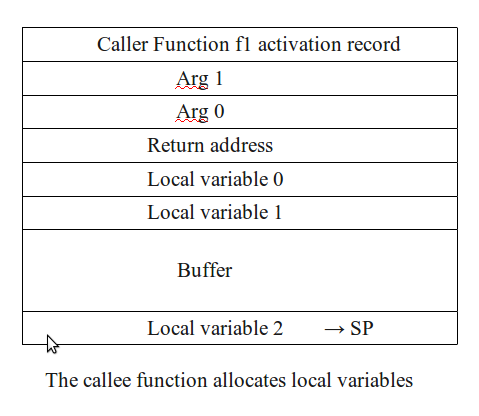
\includegraphics [width=200px,height=172px] {img/img3.png}
\end{center}
%Insert Pic here.
%Before call. After call.

\section {Return to libc Attack}
Cause buffer overflow so that the new return address of the vulnerable function
is changed to a libc function (usually system) with arguments overwritten in
such a way so as to gain unauthorized access to the system.\\
\\
For example, one can provide a shell command and overwrite the return address on
input to a webserver running as a root process to begin a root shell.  In this
way, an attacker can make use of the machine code in text section to attack a
machine irrespective of NX bits. 

\subsection {Attack}
%insert image for input.
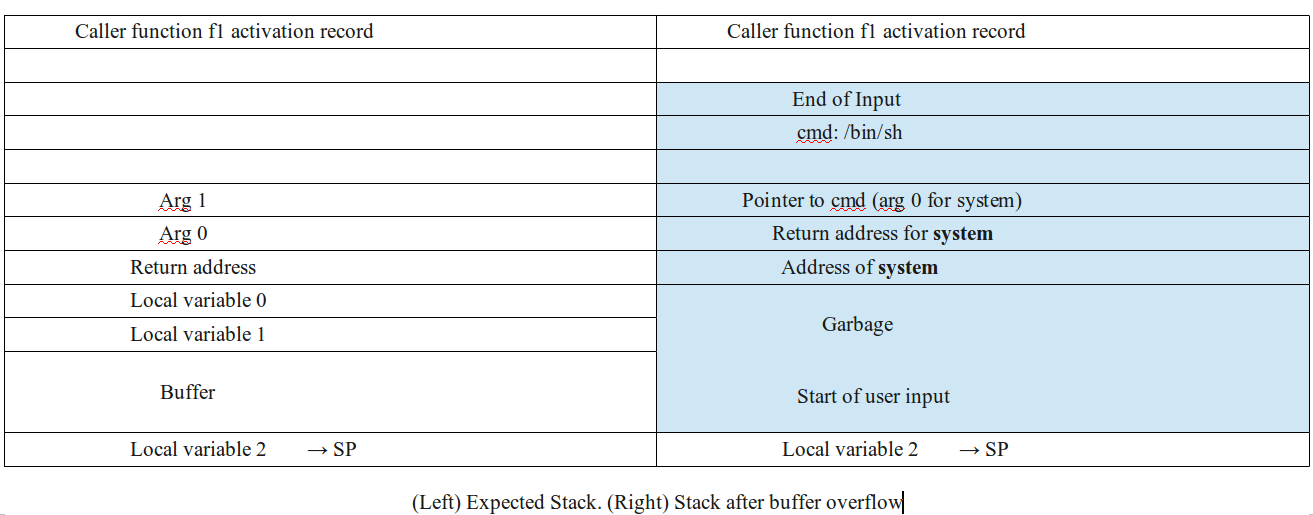
\includegraphics [width=500px,height=260px] {img/img4.png}

%Insert call sequence in return to libc attack
\subsection {How to find address of system function?}
Libraries are loaded only at page boundaries. Within a library the relative
position of a function is the same in the address space. By searching a limited
number of such page boundaries and finding the correct offset, one can locate
the system function' address.

\subsection {How to prevent?}
\begin {itemize} \itemsep -2pt
\item Not loading system function to libc if the text section of a process
does not call this.
\item Address Space Randomization.
\end {itemize}

\section {Return to libc Attack in Practical Machines}
Some real machines, expect the arguments to be placed in special registers 
(like RDA, RDB, etc) and not in stack. In such machines attackers are forced to
place the arguments in RDA by exploiting gadgets, such that by the time, control
goes to the overwritten address, RDA has the desired arguments.

\subsection {Gadget}
A gadget is a basic block of machine code, usually without a branch till it
returns. For our example attack, we consider the below gadget code, which pops
the stack pointer into the RDA register. When gadget is executed, no activation
record is pushed to stack and the stack is usually not changed. Only the IP is changed.

\begin{verbatim}
     pop %rda
     ret
\end{verbatim}

Using the gadgets, the trick is to overwrite the return address with the
address of the above gadget, followed by the argument's address (so that the
gadget copies the argument pointed by SP to RDA). This is followed by the overwriting
the return address after gadget's execution to system function's address as
usual.

\subsection {Attack}
\begin{center}
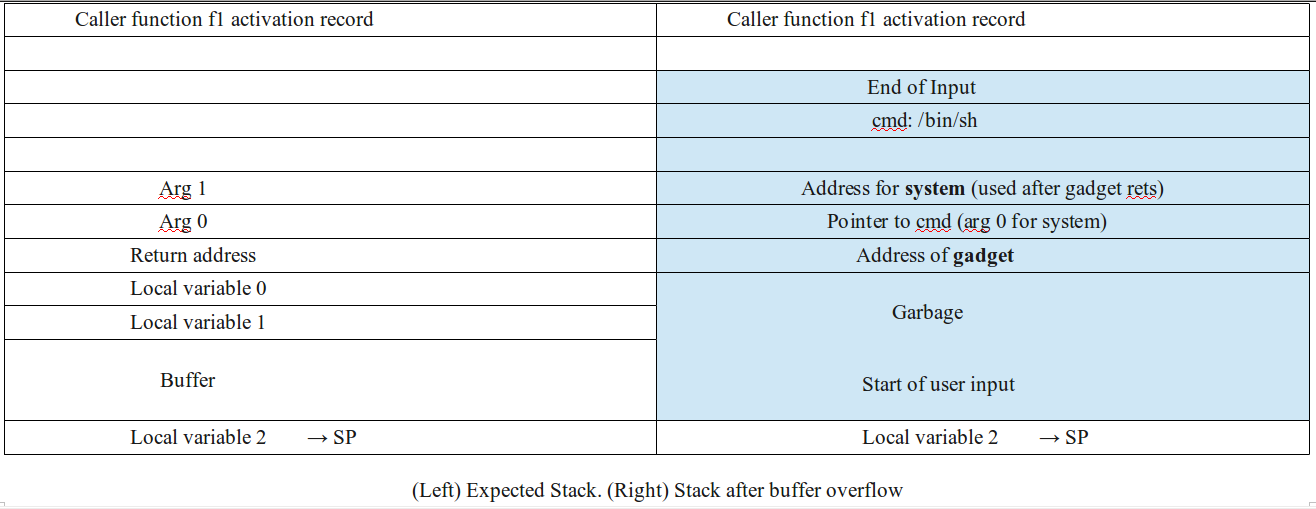
\includegraphics [width=500px,height=260px] {img/img5.png}
\end{center}

\section {Return Oriented Programming}
Return oriented programming enables us to perform arbitrary computations even
in machines with NX bit. It involves,
\begin {itemize}  \itemsep -2pt
\item Loading registers.
\item Computing addresses (by changing the return address to middle of an instruction word)
\item Inserting code off the stack.
\item Making use of gadgets (exploit the fact that gadgets have fewer instructions before ret and x86 machines have variable length instructions).
\end {itemize}

To achieve our aim of loading RDA register with the desired argument, we find
a suitable gadget which has the instruction for loading RDA as a substring in
its code. Consider the following gadget snippet.

\begin{verbatim}
     0x400006:f7c7000000 test 0x007 %edi
     0x40000B:0f9545c3   set setnzb -61 (%edi)
\end{verbatim}

Whenever the gadget is invoked the jump is to $0x400006$. But we can invoke the
gadget by following the same trick to change the return address of a vulnerable
function. But instead jump to $0x400007$, causing the machine to treat the second
byte of the gadget as the first one thus wrongly interpreting the instructions.

\begin{verbatim}
     0x400007:c70000000f movi
     0x40000B:95         xchg RDA, SP
     0x40000C:45         inc
     0x40000C:c3         ret
\end{verbatim}

We can look through the gadgets for instructions to copy to RDA ($95$ in this
example) and ret ($c3$) and change the jump address to choose a suitable
gadget to exploit for the attack. That gadgets are short and thus assist attackers to
execute the attack code and return quickly.
\end{document}
